\documentclass[a4paper,titlepage]{artikel1}
\usepackage[dutch]{babel}
%\usepackage{a4wide}
%\usepackage{eurofont}


\usepackage{ucs}
\usepackage[utf8x]{inputenc}
\usepackage{fullpage}
\usepackage{url}
\usepackage{eurosans} 
\usepackage{multirow}
\usepackage{graphicx}

\setlength{\parskip}{0.2cm}
\setcounter{secnumdepth}{3}


\author{Paul Sohier 0806122\\Sebastiaan Polderman 0820738}
\title{Automatisering}


\begin{document}
\maketitle
\tableofcontents
\newpage
 \section{Week 1}
  \subsection{Opdrachten bij hoofdstuk 1}
   \subsubsection[Opdracht 1]{Geef voorbeelden van computerprogramma's die voornamelijk ontwikkeld worden volgens het watervalmodel}
   Een pakket als MS Office zou volgens dit model ontwikkeld worden omdat het van te voren bepaalde eisen heeft aan de functionaliteit. 
   Zodra het basis pakket ontwikkeld is zal er niet veel meer veranderd worden aan het uitendelijke doel van het programma. Een uitzonder is hierop dan weer wanneer het complete pakket herschreven zal worden. Dit zal echter niet vaak gebeuren, omdat dit betekend dat je een groot aantal werkuren welke besteed zijn aan het project/programma opnieuw moet gebeuren, terwijl je uiteindelijk op dezelfde functionaliteit uitkomt. Wat wel gebeurd is dat er extra functionaliteit kan worden toegevoegd aan het programma, of bijvoorbeeld een nieuwe User Interface wordt ontwikkeld voor het programma. Op deze manier werken ze nog steeds volgens het watervalmodel, ze passen tenslotte niks aan aan de eisen voor functionaliteit.
   
   \subsubsection[Opdracht 2]{Geef voorbeelden van computerprogramma's die voornamelijk ontwikkeld worden met prototyping.}
   Een goed voorbeeld hierbij is een project op school. Hierbij wordt eigenlijk bijna direct begonnen met het werken aan het eindproduct, terwijl er nog niet echt bedacht is wat het eindproduct moet worden. Op diverse punten tijdens de ontwikkeling van het programma zal het eisenpakket worden aangepast naar de uiteindelijke wensen. In een hoop gevallen zie je bij dit soort projecten op school ook dat het eisenpakket compleet wordt overgeslagen, en er gewoon zo los gewerkt wordt. Hierbij zijn de eisen eigenlijk hetgeen waar het uiteindelijk product aan voldoet en niet zoals het van te voren is omschreven. 
   
   \subsubsection[Opdracht 3]{Wat is het verschil tussen validatie en verificatie}
   Bij validatie (Valideren) wordt gekeken of het ontwerp voldoet aan het eisenpakket, terwijl er bij verificatie wordt gekeken of het process voldeed. Het kan dus zijn dat bij het valideren het ontwerp voldoet, terwijl de verificatie zegt dat het process niet goed is verlopen, of omgekeerd. 
   
   \subsubsection[Opdracht 4]{Hoe zou u de ontwikkeltrajacten van het waterval-, het incremenetele- en het evolutionare model aangeven in figuur 1.1?}
   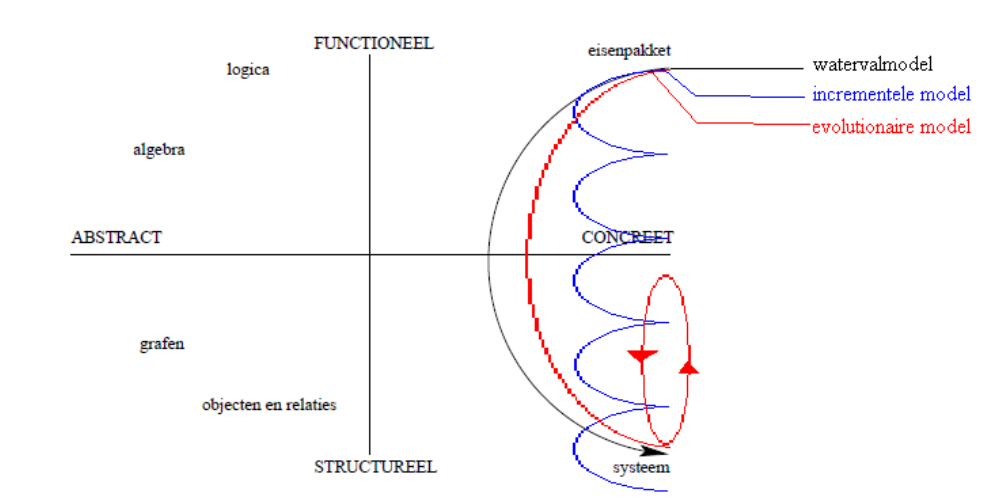
\includegraphics[scale=0.5]{H1O4.png}
   Bij het watervalmodel is duidelijk te zien dat het eerst naar het abstracte gaat voordat het systeem echt ontwikkeld wordt. Hierbij wordt dus duidelijk eerste naar het eisenpakket gekeken, en daarna pas gewerkt aan het systeem zelf. \\
   Bij het evolutionare systeem zie je ook dat er ligt wordt gewerkt naar het abstracte van het systeem, maar zie je ook dat zodra er een deel klaar is weer wordt teruggegaan van het structurele van het systeem naar het concrete en weer terug.\\
   Als laatste bij het incrementele model zie je dat er iedere keer een klein stukje abstract wordt gemaakt welke dan ontwikkeld wordt, en hierna weer doorgaat naar het abstracte om verder te ontwikkelen. Dit blijft iedere keer doorgaan tot er op een gegeven moment bij het eind een eindproduct is. Het is ook mogelijk in dit geval dat er uiteindelijk geen eindproduct is, maar de ontwikkeling steeds maar door blijft gaan.
   
   \subsubsection[Opdracht 5]{Zal de evolutionare ontwikkelstrategie de grens tussen ontwikkeling en onderhoud laten verdwijnen?}
   Ja, zodra je onderhoud doet kan je tegelijkertijd ook nieuwe, door de klant gewenste, features kunnen toevoegen aan het al bestaande programma. Hierdoor is zowel voor de klant als voor de ontwikkelaar eigenlijk niet meer te zien welk deel van de aanpassingen welke gedaan worden aan het bestaande programma nu eigenlijk onderhoud is en welk deel nu eigenlijk nieuwe features zijn. Dit kan voor beide partijen verwarring geven doordat ze niet weten of een bepaald onderdeel nu zomaar toegevoegd kan worden. Een betere methode om te gebruiken is een ontwikkel branch, en een onderhouds branchs, waarbij de wijzigingen in de onderhouds branch ook worden samengevoegd in de ontwikkelings branch (Automatische of met de hand. Door gebruik te maken van versie beheer systemen zoals SVN of GIT is dit zeer eenvoudig te doen). Zodra de ontwikkelingsbranch goed werkt, en de klant hiermee akkoord gaat kan die samengevoegd worden in de ontwikkelingsbranch welke dan de live applicatie mee kan worden ge\"{u}pdate worden. Op deze manier weet zowel de ontwikkelaar als de klant wat de status is van de huidige live branch en onderstaat er geen verwarring.
   
   \subsubsection[Opdracht 6]{Zoek op internet voorbeelde van repositories.}
   Een voorbeeld hiervan zijn de door Debian gebruikte repositories, waaruit alle Debian installaties software vandaan installeren. In deze repositories staat de al gecompileerde software opgeslagen voor de door de gebruiker gebruikte port, en kan eenvoudig worden gedownload van deze repositories en daarna geistalleerd. Op deze manier zijn updates naar de gebruiker eenvoudig uit te voeren doordat de gebruiker direct kan zien welke versie nieuw is bij het ophalen van het index bestand van het repositorie. Het nadeel van het gebruik van dit soort repositories is dat wanneer de gebruiker iets wilt wijzigen aan de compiliatie opties van de gebruikte software hij dit niet zomaar kan doen. Wanneer hij dit toch wilt doen zal hij zelf een eigen repositorie op moeten zetten en dan de software compilen en inpakken. Door een eigen repositorie te gebruiken kan de gebruiker nog steeds eenvoudig gebruik maken van de voordelen van het gebruik van een repositorie terwijl hij qua tijd niet voor meer tijd kwijt is als het los compileren van een programma. Wanneer de software echter op maar \'{e}\'{e}n installatie gebruikt wordt met de aangepast opties is het sneller/makkelijker om toch deze los te compileren en er niet een eigen pakket van te maken. \\\\
   Een ander goed voorbeeld van een repositorie is het gebruik van versie controle systemen, zoals git of svn. Dit soort systemen slaan in een repositorie op welke bestanden aanwezig zijn en wie welke wijziging gedaan heeft. Door gebruik te maken van een VCS kan een groep ontwikkelaars eenvoudig samenwerken aan dezelfde bestanden. Het VCS systeem zorgt ervoor bij eventueele conflicten dat de gebruiker gewaarschuwd wordt en deze, indien automatische samenvoeging niet werkt, moet samenvoegen. De verschillende systemen hebben allemaal hun eigen voor en nadelen bij gebruik en de keuze van de systemen hangt dus grotendeels af van wat de voorkeur van de gebruikers is. Ze hebben allemaal wel als doen om op te slaan wie welke wijziging wanneer heeft uitgevoerd.
   
   \subsubsection[Opdracht 7]{Geef de voor en nadelen van open-source software.}
   Een groot voordeel is dat de sourcecode van de applicatie/programma vrijelijk te bekijken is. Hierdoor zie je dat bijvoorbeeld security problemen welke in deze source code aanwezig zijn sneller gevonden worden en hierdoor het algemener bekend is of software veilig is of niet.
   \\
   Helaas is dit grote voordeel ook direct een nadeel. Wanneer een security probleem gevonden wordt in een applicatie/programma en dit wordt niet opgelost door de vendor kan dit makkelijk misbruikt worden door de vaak uitgebreide verspreiding van de software. 
   \\ 
   Om dit probleem in het geheel op te lossen zal je dus een combinatie moeten maken tussen veilig gebruik van software (Kijkend naar de geschiedenis van software) en ander soort software. Je kan hierbij bijvoorbeeld ook nog kijken of de software vendor patches accepteert van derden, waardoor je zelf wijzigingen kan doorvoeren en deze uitendelijk in het orginele product opgenomen worden. Dit heeft grote voordelen voor zowel de software vendor als de gebruiker.
   
   \subsubsection[Opdracht 8]{De eis ''Alle uitvoer moet normaal binnen 10 seconden gegeven worden'' is om \'{e}\'{e}n van de volgende redenen fout. Welke?}
   \begin{itemize}
    \item[a] Dubbelzinnig
    \item[b] Niet concreet
    \item[c] Tegenstrijdig
   \end{itemize}
   De eis is niet concreet genoeg, doordat alle uitvoer heel algemeen is. De programmeur heeft dus met de huidige eis geen idee wat verstaan wordt onder alle uitvoer. Dit kan bijvoorbeeld alleen zijn dat de bestelling geplaatst is, maar ook dat de bestelling direct verzonden is. \\Een verbetering op deze eis zou zijn:\\
   ''De klant moet binnen 10 seconden een bevestiging van zijn bestelling op het scherm zien.''\\
   Met deze nieuwe eis kan de programmeur zijn wat de eis is wat de klant te zien moet krijgen en dan ook daadwerkelijk dit programmeren. Zo zal er nooit een tegenstrijdigheid zijn tussen de programmeur en de opdrachtgever, want er staat duidelijk in de eis wat er moet zijn.
   
   \subsubsection[Opdracht 9]{Wat mankeert er aan de eis: ''Het bestand moet een afsluitteken bevatten.''?}
   De eis is onduidelijk, doordat het afsluitteken niet is vastgesteld in de eis. De programmeur kan dus niet simpel voldoen aan de eis zonder contact op te nemen met de opdrachtgever om te vragen wat er precies gedaan moet worden. Om de eis correct op te stellen moet het afsluitteken vermeld worden in de eis, wanneer deze wel aanwezig is kan de programmeur direct werken met de eis zonder verdere handelingen te moeten verichten om de opdracht uit te kunnen voeren.
   
   \subsubsection[Opdracht 10]{Welke maatregelen kunnen positief of negatief werken op:}
   \begin{itemize}
    \item[a] De correctheid
    \item[b] De beschikbaarheid
    \item[c] De herstelbaarheid
   \end{itemize}
   \begin{itemize}
     \item[a] Regelmatige validatie en verificatie tijdens alle stappen van het project. Hiermee wordt er gecontroleerd of de tot dan toe ontwikkelde programma's voldoen aan de gestelde eisen door de opdrachtgever.
     \item[b] Het systeem zo laten functioneren dat, mocht er een storing plaatsvinden in een bepaald gedeelte, dat de rest van het systeem nog naar behoren blijft functioneren. Hierbij kan gedacht worden aan testen in een gesimuleerde omgeving en aan testen in een real live omgeving zonder dat de omgeving dan ook echt gebruikt wordt. Ook monitoring is hierbij belangerijk, zodra de omgeving daadwerkelijk in gebruik is.
     \item[c] Optimalisatie van de programmatuur. 
   \end{itemize}
   
 \section{Week 2}
  \subsection{Opdrachten bij hoofdstuk 3}
   \subsubsection[Opdracht 1]{De projectkosten worden begroot op
   100000 euro. De winst wordt gesteld op $15\%$.Het risico dat men met dit
   project denkt te lopen, is gebaseerd op de ervaring dat $20\%$ van dit
   soort projecten mislukken. De BTW bedraagt $19\%$. Hoeveel is de
   aanbestedingsprijs?}
   \begin{displaymath}
    (100.000,00*1,15*1,2)*1,19={164.220,00}euro
   \end{displaymath}
   
   \subsubsection[Opdracht 2]{Wat zijn de verschillen tussen kosten en investeringen?}
   Kosten zijn uitgaven die direct van de winst mogen worden afgetrokken. Investeringen daarintegen moeten over meerdere jaren worden afgeschreven. Die jaarlijkse afschrijvingen mogen wel als kosten worden opgevoerd.
   
   \subsubsection[Opdracht 3]{Noem 3 investeringscriteria}
   \begin{itemize}
    \item Maximale gemiddelde boekhoudkundige rendabiliteit
    \item Minimale terugverdienperiode
    \item Concurrentievoordeel krijgen
   \end{itemize}
   \subsubsection[Opdracht 5]{Men kan een productiemiddel huren voor de
   prijs van 6100 e per maand. Indien men dit productiemiddel voor
   120000 e aanschaft, moet men 100 e per maand onderhoud betalen. De
   restwaarde is nihil.
   \begin{itemize}
     \item Bepaal het omslagpunt.
     \item Bereken het omslagpunt indien de discontovoet $1\%$ per maand is.
     \item Welke financiele overweging kan bij deze keuze een belangerijke rol spelen?
   \end{itemize}
   }
    \begin{itemize}
     \item Het omslagpunt:
	   \begin{displaymath}
	    \frac{120000}{(6100-100)}=20
	   \end{displaymath}
	   \\Het omslagpunt ligt dus bij 20 maanden
     \item Het omslagpunt bij een discotovoet van $1\%$ per maand
	   \begin{displaymath}
	    120000*1.01^{-20}=98345.34
	   \end{displaymath}
	   \begin{displaymath}
	    \frac{98345.34}{6100-100}=16.39
	   \end{displaymath}
	   \\
           Het omslagpunt ligt dan bij $16.39$ maanden.
     \item Welke overweging kan bij deze keuze een belangerijke rol spelen?\\De duurzaamheid of het gebruik van de inverstering. Hieruit bepaal je dan of het goedkoper is om te kopen of juist om het productiemiddel te huren.
    \end{itemize}
    
 \section{Week 3}
  \subsection{Opdrachten bij hoofdstuk 4}
   \subsubsection[Opdracht 1]{Noem minimaal 7 factoren die de individuele productiviteit be\"invloeden.}
   \begin{itemize}
    \item[1] Kennisniveau
    \item[2] Sfeer
    \item[3] Taalbeperkingen
    \item[4] Afhankelijk van hulpmiddelen
    \item[5] Budget
    \item[6] Werkprocessen
    \item[7] Beloning
   \end{itemize}
   
   \subsubsection[Opdracht 2]{Wat is het bezwaar tegen de definitie van
   individuele productiviteit: ``De omvang van de objectcode
   (gecompileerde programmatuur) in bytes per tijdseenheid''?}
   Iemand die minder efficient programeert levert volgens deze stelling beter werk af. Ook wordt er hiermee niet gekeken naar de complexiteit van de code.
   
   \subsubsection[Opdracht 3]{Verklaar waarom het coderen in de
   uitwerkingsfase meestal minder dan 10\% van de totale kosten van de levenscyclus bedraagt.}
   Door het gebruik van hulpmiddelen krimpt het coderingsaandeel.
   
   \subsubsection[Opdracht 4]{Verklaar hoe uit de COCOMO methoden blijkt dat de projecttijd niet afhankelijk is van het aantal programmeurs.}
   De geschatte projecttijd T wordt berekend door het aantal mensmaanden tot de macht c (Compactheid), vermenigvuldigt met $2,5$. Op basis hiervan wordt het minimum aantal benodigde mensen geschat. Het model rekent niet de projecttijd uit op basis van het aantal teamleden.

   \subsubsection[Opdracht 5]{Een administratief systeem van 9 netto
   functiepunten werd met een inspanning van 3 mensmaanden
   ontwikkeld. Is dit kenmerkend voor een administratief
   automatiseringsproject?}
   Volgens figuur 4.6 (Tabel \ref{reffig46}) in de reader is de gemiddelde productiviteit voor administatieve systemen $15,2$. De parameters van vraag 5 geven een productiviteit van $3$.

   \begin{center}
   \begin{table}[h] %hij zet hem op volgende pagina. Moet nog even kijken hoe beter aan te passen dat hij echt hier komt.
     \caption{Figuur 4.6}\label{reffig46}
     \begin{center}
     \begin{tabular}[t]{|l|l|l|l|}
       \hline
       \multirow{3}{*}{Toepassingsgebied} & \multicolumn{3}{c|}{Productiveit P [nfp/mensmaand]} \\
       \cline{2-4}
       & gemiddeld & standaarddeviatie & variatieco\"{e}ffici\"{e}nt \\
       & $\mu$ & $\sigma$ & $\rho$ \\
       \hline
       systemen met microcode & $1,5$ & $2,7$ & $1,80$ \\
       ingebedde realtime systemen & $6,8$ & $3,1$ & $0,46$ \\
       vliegtuigsystemen & $6,4$ & $3,3$ & $0,52$ \\
       commando en controle systemen & $9,9$ & $4,1$ & $0,41$ \\
       procesbesturings systemen & $10,3$ & $4,3$ & $0,42$ \\
       besturingsprogrammas en utilities & $11,3$ & $3,9$ & $0,35$ \\
       wetenschappelijke systemen & $12,5$ & $4,0$ & $0,32$ \\
       netwerksystemen & $10,3$ & $3,1$ & $0,30$ \\
       administratieve systemen & $15,2$ & $3,8$ & $0,24$ \\
       \hline
     \end{tabular}
     \end{center}
   \end{table}
   \end{center}
   
   \subsubsection[Opdracht 6]{Een computerprogramma heeft bij functiepuntanalyse voor de systeemkarakteristieken een totale correctiefactor $\bullet \begin{array}{c}14\\i=1 \end{array} c_i=50$. Uit de specificatie blijkt dat er 3 verschillende invoer-, 7 uitvoer- en 5 vraagtypen nodig zijn. Daarnaast zijn er 2 externe gegevensverzamelingen en 2 interne gegevensverzamelingen nodig. Alle geruiktsfuncties hebben een gemiddelde complexiteit. Men zal het computerprogramma coderen in de taal JAva ($C_t=53$). Er wordt geen gebruik gemaakt van hergebruik. Maak een schatting voor de broncode.}
   \begin{displaymath}
    f=3*4+4*5+5*4+2*10+2*7=12+20+20+20+14=86
   \end{displaymath}
   
   \begin{displaymath}
    NFP=(0,65+0,01*50)*86=98,9 %Was 1.15
   \end{displaymath}
   
   \begin{displaymath}
    S=98,9*53=5241,7
   \end{displaymath}
   Het aantal regels broncode is dus ongeveer $5241$
   \subsubsection[Opdracht 7]{Verklaar waarom juist computertalen met een lage ct waarde (zie paragraaf 4.1.1) geschikt zijn voor prototyping.}
   Dit komt doordat de hoeveelheid code kleiner is en hierdoor dus sneller is aan te passen
   
   \subsubsection[Opdracht 8]{Gegven een studentinformatiesysteem bestaande uit de volgende onderdelen:
     \begin{center}
   \begin{tabular}[t]{|ll|l|}
     \hline
     soort & omschrijving & complexiteit \\
     \hline
     module & inschrijving student & gemakkelijk \\
     module & uitschrijving student & gemakkelijk \\
     module & rekening collegegeld sturen & gemakkelijk \\
     module & machtiging betaling collegegeld verwerken & makkelijk \\
     module & betaling collegegeld verwerken & gemiddeld \\
     module & aanmaningen sturen & gemakkelijk \\
     module & tentamencijfers verwerken & moeilijk \\
     module & studieresultaten naar Informatie Beheer Groep & gemiddeld \\
     scherm & inschrijven van een student & gemiddeld \\
     scherm & uitschrijven van een student & gemiddeld \\
     scherm & betaling student invoeren & gemiddeld \\
     scherm & machtiging betaling invoeren & gemiddeld \\
     scherm & tentamencijfers invoeren & moeilijk \\
     scherm & vakkentabel invoeren & gemiddeld \\
     scherm & vakkentabel wijzigen & moeilijk \\
     formulier & studentgegevens & gemiddeld \\
     formulier & jaarlijkse voortgangsrapportage & moeilijk \\
     formulier & rapportage van tentamenresultaten & moeilijk \\
     formulier & aanmaningen collegegeld & gemiddeld \\
     \hline
   \end{tabular}
   \end{center}
   \begin{itemize}
     \item Maak met een objectpuntanalyse (OPA) een schatting voor de inspanning E als het hergebruik rond de $30\%$ ligt en het ontwikkelteam een lage productiviteit heeft. Maak een schatting met COCOMO-81 van de projecttijd T, indien het project een `organische' karakter heeft.
     \item Maak een schatting van de projecttijd T met COCOMO-II, indien er geen sprake is van tijdsdruk en het project de volgende karateristieken heeft:\\
       \begin{center}
       \begin{tabular}[]{|l|l|}
         \hline
         Karakteristieken & $b_i$ \\
         \hline
         ontwerpervaring & $0,05$ \\
         ontwerpvrijheid & $0,02$ \\
         ontwerprisico & $0,3$ \\
         ontwerpteam & $0,03$ \\
         organisatie & $0,01$ \\
         \hline
       \end{tabular}
       \\
       \end{center}
   \end{itemize}
   %\\ %Anders lijkt het antwoord op de vraag nog :)
   }
   \begin{itemize}
    \item OPA
	  \begin{displaymath}
	   NOP=50*(1-0.3)=35
	  \end{displaymath} 
	  \begin{displaymath}
	   E=\frac{35}{7}=5
	  \end{displaymath}
    \item COCOMO-81
	  \begin{displaymath}
	   T=2.5*5.2^{0.38}=4.78
	  \end{displaymath}
    \item COCOMO-II
	  \begin{displaymath}
	   T=(2.5*5.2^{0.33+0.2*0.14})=4.51
	  \end{displaymath}
   \end{itemize}
   \section{Week 4}

   \subsection{Opdrachten bij hoofdstuk 5}
   \subsubsection[Opdracht 1]{Gegeven een netwerk met 7 activiteiten:}
   \begin{center}
     \begin{tabular}{|l|l|l|l|l|l|}
       \hline
       activiteit & omschrijving & afhankelijk van & $t_b$ & $t_m$ & $t_w$ \\
       \hline
       A & Definitie & & 1 & 2 & 3 \\
       B & Hardware specificatie & A & 3 & 4 & 5 \\
       C & Software specificatie & A & 1 & 2 & 9 \\
       D & Hardware ontwikkeling & B & 1 & 2 & 3 \\
       E & Software ontwikkeling & B C & 4 & 5 & 12 \\
       F & Documenteren & D & 3 & 4 & 5 \\
       G & Systeemintergratie & D E & 3 & 3 & 3 \\
       \hline
     \end{tabular}
   \end{center}
   \begin{itemize}
     \item[a] Bepaal met PERT het mijpalenplan en het kritieke pad
     \item[b] Bepaal het Ganttscheme. Welke conclusies kan men daaruit trekken?
     \item[c] Bepaal het 95\%-betrouwbaarheidsinterval voor de werkelijke projecttijd.
   \end{itemize}
   \begin{itemize}
     \item[a] Zie figuur \ref{r51a}.
     \item[b] Zie tabel \ref{r51b}.
     \item[c]
       \begin{displaymath}
         o²=2+2+8+2=2+8+2+0=24
       \end{displaymath}
       \begin{displaymath}
         14-(1,96*\sqrt{24})=<T=<14+(1,96*\sqrt{24}))
       \end{displaymath}
       \begin{displaymath}
         4,40=<T=<26,60
       \end{displaymath}
   \end{itemize}
       \begin{figure}[tbh]
         \caption{Antwoord bij Hoofdstuk 5 Vraag 1.a} \label{r51a}
         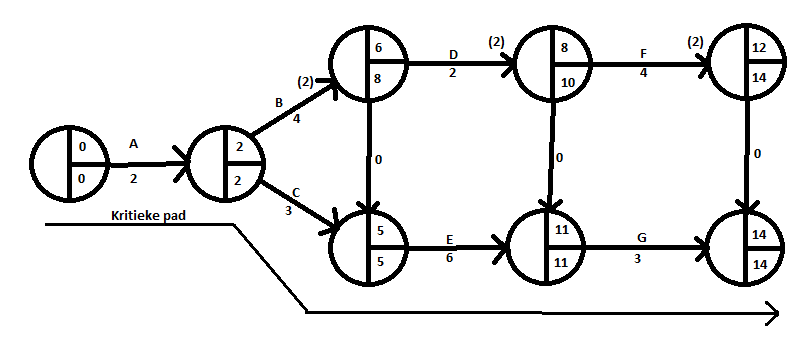
\includegraphics[scale=0.75]{H5O1A.png}     
       \end{figure}
   \begin{table}
     \caption{Antwoord bij Hoofdstuk 5 vraag 1.b} \label{r51b}
       \begin{tabular}[htb]{|l|l|l|l|l|l|l|l|l|l|l|l|l|l|l|}
         \hline
             & 0..1 & 1..2 & 2..3 & 3..4 & 4..5 & 5..6 & 6..7 & 7..8 & 8..9 & 9..10 & 10..11 & 11..12 & 12..13 & 13..14 \\
         \hline
         A 2 &  --- &  --- &      &      &      &      &      &      &      &       &        &        &        &\\
         \hline
         B 4 &      &      &  --- & ---  & ---  & ---  & - - -& - - -&      &       &        &        &        &\\
         \hline
         C 3 &      &      &  --- & ---  & ---  &      &      &      &      &       &        &        &        &\\
         \hline
         D 2 &      &      &      &      &      &      & - - -& - - -&      &       &        &        &        &\\
         \hline
         E 6 &      &      &      &      &      & ---  & ---  & ---  & ---  & ---   & ---    &        &        &\\
         \hline     
         F 4 &      &      &      &      &      &      &      &      & - - -& - - - & ---    & ---    & - - -  & - - -\\
         \hline
         G 3 &      &      &      &      &      &      &      &      &      &       &        & ---    & ---    & ---\\
         \hline
       \end{tabular}
   \end{table}
   
   \subsubsection[Opdracht 2]{bepaal van de volgend activiteiten met PERT het mijlpalenplan en een schatting van het kritieke pad $T_k$}
   \begin{center}
     \begin{tabular}{|l|l|l|}
     \hline
     activiteit & $t$ & afhankelijk van \\
     \hline
     A & 2 & K \\
     B & 3 & H \\
     C & 4 &\\
     D & 2 & F G \\
     E & 1 & D I J \\
     F & 3 & B \\
     G & 3 & C K \\
     H & 3 & \\
     I & 2 & A F \\
     J & 1 & F \\
     K & 2 & H \\
     \hline
     \end{tabular}
   \end{center}
   \subsubsection[Opdracht 3]{Van een collectief team is gegeven dat de verliesfactor per communicatiekaneel 5\% is, bereken de maximale groepsgrootte}
   \begin{displaymath}
     N=\frac{(1+i)}{(2*i)}=\frac{1+0,05}{2*0,05}=\frac{1,05}{0,10}=10,5
   \end{displaymath}

   \subsubsection[Opdracht 4]{Toon aan dat de volgende formule geldt voor het hi\"{e}rarchieke team met $N$ teamleden en maximaal 6 ondergeschikten per echelon:}
   \begin{displaymath}
     \lfloor^6\log{(5N+1)}\rfloor\leq echelons\leq N
   \end{displaymath}
   De $6$ in de log geeft aan hoeveel ondergeschikten er in een echelon zijn. Wanneer je de $6$ veranderd naar een hoger of lager getal zal de waarde van N veranderen naar een nieuw maximaal aantal wat werkbaar is binnen een team. Tevens veranderd hierin het aantal echelons ook negatief, wat betekend dat de communcatie en informatie overdracht tussen de verschillende echelons wordt vergroot. Alle informatie moet tenslotte eerste naar de bovenste echelon welke hier dan weer de informatie teruggeeft naar de ondergeschikte welke de benodigde informatie heeft bij \'{e}\'{e}n van zijn ondergeschikte. Wanneer dit niet via de bovenste echelonn zou gaan zou de bovenste echelon niet de benodigde informatie hebben welke hij nodig heeft om het project goed te kunnen leiden. Het gebruik van de hi\"{e}rarchieke structuur heeft grote voordelen bij grote projecten met veel verschillende bedrijven/onderdelen, doordat er een globaal overzicht is over hoever het project gevorderd is. Het nadeel blijft ook hier dat de informatie voorziening lastig kan zijn bij een groot aantal echelons.
   \section{Week 5}
   \subsection{Opdrachten bij hoofdstuk 7}
   \subsubsection[Opdracht 1]{Van een objectgeori\"{e}nteerd computerprogramma in Java, zijn van alle classes de metrieken NOM,CBO, RFC, WMC, DIT en NOC gemeten. Een tiental classes had een verhoogd risico.}
   \begin{itemize}
     \item[a] Maak een tabel met riskante waarden van de waarden van de metrieken.
       \begin{center}
         \begin{tabular}{|l|p{5cm}|l|l|}
           \hline
           Metrieken & Riskante waarde & reader bladzijde & reader paragraaf\\
           \hline
           NOM & Java gemiddeld: $\approx8$ & 84 & 7.2.2 \\
           & C++ gemiddeld: $\approx25$ & & \\
           & Kritiek: $>40$ & & \\
           \hline
           CBO & 5 & 86 & 7.2.5 \\
           \hline
           RFC & $\geq50$ & 87 & 7.2.7 \\
           \hline 
           RFC/NOM & Java: $\geq10$ & 88 & 7.2.7 \\
           & C++: $\geq5$ & & \\
           \hline
           WMC & aanbevolen: $\geq25$ & 83 & 7.2.1 \\
           & kritiek: $>75$ & & \\
           \hline
           DIT & 5 & 84  & 7.2.3 \\
           \hline
           NOC & Geen aanbevolen waarde, hoge NOC geeft slechte metriek & 85  & 7.2.4  \\
           \hline
         \end{tabular}
       \end{center}
     \item[b] Geef in de volgende tabel bij elke class aan welke metriek een kritieke waarde heeft. \\
       \begin{center}
       \begin{tabular}{|l|l|l|l|l|l|l|l|}
         \hline
         class & NOM & CBO & RFC & RFC/NOM & WMC & DIT & NOC \\
         \hline
         1 & 54 & 8 & 536 & 9,9 & 175 & 1 & 0 \\
         2 & 7 & 6 & 168 & 24,0 & 71 & 4 & 0 \\
         3 & 33 & 4 & 240 & 7,2 & 105 & 2 & 0 \\
         4 & 54 & 8 & 381 & 6,7& 117 & 2 & 2 \\
         5 & 62 & 6 & 378 & 6,1 & 163 & 2 & 0 \\
         6 & 63 & 7 & 235 & 3,7 & 156 & 2 & 0 \\
         7 & 81 & 10  & 285 & 3,5 & 161 & 2 & 0 \\
         8 & 42 & 5 & 127 & 3,0 & 69 & 3 & 0 \\
         9 & 20 & 17 & 325 & 16,2 & 139 & 4 & 4 \\
         10 & 46 & 5 & 186 & 4,0 & 238 & 1 & 3 \\
         \hline
       \end{tabular}
       \end{center}
       
       Bij NOC is er geen aanbevolen kritieke waarde, maar er is wel hoe hoger deze waarde is hoe slechter de metriek is. Wij hebben bij een NOC van $\geq3$ aangenomen dat de NOC kritiek is. Dit baseren wij op dat de NOC is gebaseerd op het aantal kinderen een class heeft, en hoe meer kinderen, hoe groter de kans op fout. Bij $\geq3$ is de kans op fouten volgens onze mening zeer goed aanwezig.\\
       Wanneer een waarde kritiek is voor een bepaald metriek, staat er in onderstaande tabel \begin{em}kritiek\end{em}. Wanneer er niets staat is de waarde niet kritiek. Er is uitgegaan dat de classes zijn geschreven in de taal JAVA, zoals vermeld in de opdracht. Echter indien de waarde uitmaakt in welke taal (JAVA of C++) de class is geschreven voor de kritieke waarde, staat de waarde voor C++ tussen haakjes. \\ 
         De waarde voor RFC is in alle gevallen kritiek. De waarde ligt flink boven de aangegeven kritieke waarde, welke tevens ook zeer hoog boven de kritieke waarde ligt. De kritieke waarde voor RFC ic $\geq50$, terwijl de laagste waarde voor RFC van de classes 127 is. \\
         De waarde voor DIT ligt in alle gevallen onder de kritieke waarde van 5. 
       \begin{center}
       \begin{tabular}{|l|l|l|l|l|l|l|l|}
         \hline
         class & NOM & CBO & RFC & RFC/NOM & WMC & DIT & NOC \\
         \hline
         1 & kritiek & kritiek & kritiek & (kritiek) & kritiek &  &  \\
         2 &  & kritiek & kritiek & kritiek(kritiek) &  &  &  \\
         3 &  &  & kritiek & (kritiek) & kritiek &  & \\
         4 & kritiek & kritiek & kritiek & (kritiek)& kritiek &  &  \\
         5 & kritiek & kritiek & kritiek & (kritiek) & kritiek &  &  \\
         6 & kritiek & kritiek & kritiek &  & kritiek &  &  \\
         7 & kritiek & kritiek  & kritiek &  & kritiek &  &  \\
         8 & kritiek & kritiek & kritiek &  &  &  &  \\
         9 &  & kritiek & kritiek & kritiek(kritiek) & kritiek &  & kritiek \\
         10 & kritiek & kritiek & kritiek &  & kritiek &  & kritiek \\
         \hline
       \end{tabular}
       \end{center}

   \end{itemize}
   
   \subsubsection[Opdracht 2]{Bepaald WMC, DIT, NOC, CBO, RFC en LCOM van de volgende pseudo objecten broncode:}
   \begin{center}
   \begin{tabular}{|l|l|}
     \hline
     Class & trade \\
     Variables & trade.id, counterparty, trade\_value \\
     Methods & evaluate\_counterpart() \\
     & get\_trade\_id(trade\_id) \\
     & position\_update() \\
     & \{position\_manager::report\_trade()\} \\
     \hline
     Class & bond\_trade \\
     Variables & bond\_detials \\
     Methods & get\_bond\_info() \\
     \hline
     Class & fx\_trade \\
     Variables & forex\_detials \\
     Methods & calculate\_exchange\_rates() \\
     \hline
     Class & equity\_trade \\
     Variables & company, stock\_market, PE\_ratio,  earnings, week\_hi\_lo \\
     Methods & Estimate\_beta() \\
     & get\_stock\_quotes() \\
     & \{quotron::quotes()\} \\
     \hline
     Class &municipal\_bond\_trade \\
     Variables & state\_or\_federal, over\_the\_counter \\
     Methods & calculate\_coupon\_rate() \\
     & \{Tbil\_server::rate()\} \\
     \hline
     Class & corporate bond\_trade \\
     Variables & adr, sp\_rating \\
     Methods & calc\_rating(sp\_rating) \\
     & \{if adr then fx\_trade::calculate\_exchange\_rates()\} \\
     \hline
     Class & international\_equity \\
     Variables & exchange\_rate, quitation \\
     Methods & perform\_anaylysis\_roa()\\
     & \{fx\_trade::calculate\_exchange\_rates()\}\\
     & get\_quotron(quotation) \\
     \hline
     Class & domestic\_equity \\
     Variables & variables: attribute1\\
     Methods & \\
     \hline
   \end{tabular}
   \end{center}
   In de tabel hieronder staan alle waarde voor de verschillende metrieken. Onder de tabel staat de uitleg erbij met de berekening van de verschillende metrieken. Tevens staat in de tabel hieronder of de waarde kritiek is voor het type metriek.
   \begin{center}
     \begin{tabular}{|l||l|l|}
       \hline
       Metriek & Waarde & Kritek \\
       \hline
       WMC & 11 & Nee \\
       \hline
       DIT & Zie hieronder & \\
       \hline
       NOC & Zie hieronder & \\
       \hline
       CBO & 4 & Nee, maar zie hieronder\\
       \hline
       RFC & 16 & Nee, maar zie hieronder \\
       \hline
       LCOM & Zie hieronder & \\
       \hline
      \end{tabular}
   \end{center}
   \begin{center}\begin{bf}WMC\end{bf}\end{center}
   WMC houd in dat er voor iedere methode in een class 1 wordt geteld. Voor iedere routine in die methode word daarbij nog 1 opgeteld. Er is in dit geval maar bij één class in een methode een routine aanwezig.
   \begin{bf}Class trade\end{bf}\\
     De WMC van de class trade is als volgt:
     \begin{itemize}
       \item 3 methodes: 3
       \item Geen routines
     \end{itemize}
     De WMC van de class trade is 3.\\
   \begin{bf}Class bondtrade\end{bf}\\
     De WMC van de class bondtrade is als volgt:
     \begin{itemize}
       \item 1 methode: 1
       \item Geen routines
     \end{itemize}
     De WMC van de class bondtrade is 1.\\
    \begin{bf}Class fx\_trade\end{bf}\\
    De WMC van de class fx\_trade is als volgt:
    \begin{itemize}
      \item 1 methode: 1
      \item Geen routines
    \end{itemize}
    De WMC van de class fx\_trade is 1.\\
    \begin{bf}Class equity\_trade\end{bf}\\
    De WMC van de class equity\_trade is als volgt:
    \begin{itemize}
      \item 2 methodes: 2
      \item Geen routines
    \end{itemize}
    De WMC van de class equity\_trade is: 2.\\
    \begin{bf}Class municipal\_bond\_trade\end{bf} \\
    De WMC van de class municipal\_bond\_trade is als volgt:
    \begin{itemize}
      \item 1 methode: 1
      \item Geen routines
    \end{itemize}
    De WMC van de class municipal\_bond\_trade is: 1.\\
    \begin{bf}Class corporate\_bond\_trade\end{bf}\\
    De WMC van de class corporate\_bond\_trade is als volgt:
    \begin{itemize}
      \item 1 methode: 1
      \item 1 routine: 1
    \end{itemize}
    De WMC van de class corporate\_bond\_trade is: $1 + 1 = 2$.\\
    \begin{bf}Class international\_equity\end{bf}\\
    De WMC van de class international\_equity is als volgt:
    \begin{itemize}
      \item 1 methode: 1
      \item geen routines
    \end{itemize}
    De WMC van de class international\_equity is: 1\\
    \begin{bf}Class domestic\_equity\end{bf}\\
    De WMC van de class domestic\_equity is als volgt:
    \begin{itemize}
      \item Geen methode
      \item geen routines
    \end{itemize}
    De WMC van de class domestic\_equity is: 0 \\
    \begin{bf}Totale WMC\end{bf}\\
      De totale WMC is als volgt: \\
      \begin{displaymath}
        3 + 1 + 1 + 2 + 1 + 2 + 1 = 11
      \end{displaymath}
   \begin{center}\begin{bf}DIT\end{bf}\end{center}
    DIT houd in dat er wordt gekeken naar de overerving van classes. Hierbij wordt het aantal ouders geteld wat een bepaalde class is. De DIT hoort niet hoger te zijn als 5 voor een bepaalde class. Bij de DIT wordt puur per class gekeken, en niet zoals bij de WMC naar het totaal. In het geval van de opgegeven pseude code is niet duidelijk uit te halen welke classes een ouder hebben, en wat de ouder dan ook is. Hierdoor is het niet mogelijk de DIT van de classes te berekenen. Mogelijk dat alle classes in dit geval super classes (Ofwel zonder ouders zijn). Dit betekend echter wel dat de classes slecht zijn opgebouwd. Maar ook hiervoor is geen direct bewijs uit de pseude classes te halen. 
   \begin{center}\begin{bf}NOC\end{bf}\end{center}
   NOC geeft een indicatie wat een bepaalde class voor uitoefining heeft op zijn kinderen. Hierbij geeft een hoge NOC aan dat de classes slechter te testen zijn. Er is geen vaste waarde voor de NOC welke slecht is, maar een hogere NOC kan problemen opleveren. Net als bij de DIT is de NOC afhankelijk van de kinderen/ouders. Doordat dit niet is aangegeven in de pseudocode is het niet te berekenen wat de NOC is. Mogelijk zijn er geen kinderen, en is de NOC 0.
   \begin{center}\begin{bf}CBO\end{bf}\end{center}
   Bij CBO wordt gekeken naar afhankelijkheid van andere classes welke niet door overerving gekoppeld zijn. Doordat in dit geval geen relates zijn opgegeven in de pseude code gaan we ervan uit dat alle methode calls welke uitgevoerd worden niet door overerving zijn bedoeld. De volgende classes hebben geen methode calls buiten hun eigen class, en de CBO is dus 0:
   \begin{itemize}
     \item bond\_trade
     \item fx\_trade
     \item dometic\_equity
   \end{itemize}
   De volgende classes hebben allemaal \'{e}\'{e}n methode call buiten hun eigen class:
   \begin{itemize}
     \item equity\_trade
     \item municipal\_bond\_trade
     \item corporate\_bond\_trade
     \item international\_equity
   \end{itemize}
   De CBO van de classes is totaal bij elkaar dus 4. De CBO hoort in principe $<5$ te zijn, algemeen aangenomen. Dit is het geval in de bovenstaande classes. Bij een hogere CBO wordt de koppeling groot, en is de modulariteit van het ontwerp in het geding. Dit kan betekenen dat de classes lastig te zijn hergebruiken, terwijl juist de bedoeling van het gebruik van classes is dat deze goed te zijn hergebruiken. In bovenstaand voorbeeld kom ik in dit geval tot een andere conclusie. Doordat er, zover te zien in de pseudecode, geen overerving is, zijn alle classes afhankelijk van elkaar, dit zorgt er in dit specifieke geval dus voor dat \'{e}\'{e}n losse klas eigenlijk helemaal niet makkelijk los te gebruiken is. Dit komt doordat de CBO gemaakt is voor grotere stukken code, terwijl het voorbeeld hier zeer minimaal is. Volgens de standaard is de code dus eigenlijk niet kritiek, maar ik durf te zeggen dat deze dat wel is.
   \begin{center}\begin{bf}RFC\end{bf}\end{center}
   De RFC telt het aantal methode in een class, plus het aantal externe methode welke aangeroepen worden. Het resultaat van de metriek is de intensiviteit van de communicatie met andere classes. Het is aan te raden om de RFC op $\leq50$ te houden. Hierboven wordt de waarde van de complexiteit te hoog waardoor het lastig wordt om de class te wijzigen en de class te snappen.
   \\
   De volgende classes hebben geen externe methode welke aangeroepen. Hierbij is de RFC van die class gelijk aan het aantal methode:
   \begin{itemize}
     \item bond\_trade: 1 methode
     \item fx\_trade: 1 methode
     \item domestic\_equity: 0 methodes
   \end{itemize}
   De RFC van deze 3 classes is dus bij elkaar 2.
   De volgende classes hebben naast normale methode ook methode welke extern aangeroepen worden. Hierbij is de RFC van die class gelijk aan het aantal methoden plus het aantal extern aangeroepen methoden. Het aantal externe methodes welke aangeroepen worden is in alle gevallen \'{e}\'{e}n.
   \begin{itemize}
     \item trade: 3 methodes
     \item equity\_trade: 2 methodes
     \item municipal\_bond\_trade: 1 methode
     \item corporate\_bond\_trade: 1 methode
     \item international\_equity: 2 methodes
   \end{itemize}
   In totaal is de RFC voor deze 5 classes: $3 + 2 + 1 + 1 + 2 + 5 = 14$. De $5$ in de berekening komt van de extern aangeroepen methode.
   In totaal is de RFC van alle classes totaal $2 + 14 = 16$. De kritieke waarde voor RFC van classes is $\leq50$, en volgens de eigenlijke standaard is de RFC niet kritiek. Maar net als bij de CBO durf ik te stellen dat in dit geval de pseudo code niet duidelijk genoeg is, waardoor de eigenlijke complexiteit van de classes toch te hoog is, terwijl de RFC toch binnen de aangegeven waarde valt. Wanneer er duidelijker in de pseudecode wordt aangegeven wat de exacte classes zijn, en wanneer deze ook duidelijke referenties aangeven kan er een betere conclusie worden getrokken uit de waarde.
   \begin{center}\begin{bf}LCOM\end{bf}\end{center}
   De LCOM geeft aan in hoeveel een class met elkaar in verband staan. Hierbij wordt gekeken naar de gemeenschappelijk object variable. Hoe lager de LCOM, hoe beter de class samenwerkt. Wanneer de LCOM te hoog is, is de samenhang niet goed en moet de class eigenlijk gesplitst worden in meerdere losse classes. In het meest gunstige geval is de LCOM $\leq1$, wat een goede samenhang betekend.\\Doordat de pseudecode niet aangeeft welke object variable gebruikt worden in een bepaalde methode is het niet te doen om de LCOM te berekenen. Om de LCOM te kunnen berekenen zal er in de pseudocode moeten worden weergeven welke object variable er in die methode gebruikt wordt.
   \begin{center}\begin{bf}Conclusie\end{bf}\end{center}
   Zoals hierboven al geschreven kunnen de DIT, NOC en LCOM niet berekend worden doordat de vereiste gegevens missen in de pseudo code. Wanneer de vereiste gegevens wel gegeven waren konden deze drie metrieken vrij eenvoudig berekend worden. Echter, om tot een goed resultaat te komen, zoals bij een normaal project echt gebruikt wordt zal de code welke gebruikt wordt om deze opdracht te maken flink uitgebreid moeten worden. De huidige resultaten uit de diverse metrieken komen niet goed overeen met de eigenlijke complexiteit van de gegeven code. Dit komt doordat de code welke aanwezig is zo klein is dat je weinig complexiteit ziet in de metrieken. Maar wanneer je gaat kijken naar de diverse methode en classes hoe ze in elkaar zitten zie je dat alle classes eigenlijke afhankelijk zijn van elkaar. Om deze redenen zijn de classes dus niet correct opgebouwd en kan de opgegeven classes niet hergebruiken, terwijl dit uitendelijk wel het orginele doel is van het gebruik van classes. Om dit toch te kunnen bewerkenstellen zouden alle aanwezige classes welke er zijn herschreven moeten worden, zodat ze data welke universeel is accepteren. Tevens zouden de extern aangeroepen methode verkleint moeten worden met het huidige aantal. Wanneer dit gebeurd is zulleen de classes uit de pseudocode niet alleen beter uit de verschillende metrieken komen, maar ook beter herbruikbaar zijn voor de verschillende opdrachten.
\end{document}
